\documentclass{bfh}

\title{Project 2}
\subtitle{Bitmessage -- Communication Without Metadata}
\author{Christian Basler}
\tutor{Kai Brünnler}
\date{\today}

\begin{document}
  \maketitle

  \tableofcontents

  \section{Synopsis}

  TODO


  % Section basics
    \section{Einführung}

  \subsection{Was sind Metadaten?}

  Metadaten sind informationen, welche als Nebeneffekte der eigentlichen Kommunikation auftreten. Wer schreibt wem? Wann? Über welchen Kanal?

  Verschlüsselungstechnologien wie PGP oder S/MIME ermöglichen uns auf sichere Art und Weise Nachrichten vor neugierigen Augen zu schützen. Doch seit Edward Snowden den NSA-Skandal aufgedeckt hat wissen wir, dass Metadaten --- vor allem Informationen darüber wer mit wem kommuniziert -- genauso interessant und viel einfacher zu analysieren sind.

  Es gibt einige Beispiele wie Sie durch Metadaten in Schwierigkeiten kommen können. Wenn Sie jemandem schreiben der in der IS ist, kann es durchaus sein, dass Sie das nächste mal nicht in die USA fliegen können. Die No-Fly-Liste kümmert sich dabei nicht darum dass Sie Journalist sind oder keine Ahnung hatten dass diese Person ein Terrorist war.

  \subsection{Wie können wir Metadaten verstecken?}

  Mit E-Mail können wir die Verbindung zu unserem Mail-Provider verschlüsseln und dieser wiederum die Verbindung mit dem Provider unseres Gesprächspartners. Dabei können wir nur hoffen, dass unser Anbieter und derjenige des Empfängers sowohl vertrauenswürdig als auch kompetent sind.\footnote{Gratis sollte er natürlich auch noch sein.}

  Bei Bitmessage senden wir eine Nachricht an eine grosse Anzahl Teilnehmer, darunter den eigentlichen Empfänger. Die Nachricht ist dabei so verschlüsselt, dass nur der Besitzer des privaten Schlüssels diese lesen kann. Alle Teilnehmer versuchen nun, alle Meldungen zu entschlüsseln, um so die für sie bestimmten Nachrichten zu finden.

  The protocol is described in detail in my Seminar paper.


  \section{Goal}

  At the moment, there aren't many implementations apart from the official clients. Especially two things are missing: a multi purpose Java library and a usable mobile client. My goal for my \textit{Project 2} is to create the library, to be used next semester as a starting point for an Android\textsuperscript{\texttrademark} client in my Bachelor Thesis.


  \section{Issues}

  TODO


  \subsection{Unsigned Numbers}

  Java doesn't support unsigned number types. While Java 8 has some helper classes to address this issue, my goal is to support Java 7, which is needed for Android development, so I wasn't able to leverage them.

  \subsection{Proof of Work}

  Proof of work is needed for a message to be distributed within the Bitmessage network. This is to protect both the network itself from denial of service attacks and the users from spam.


  \section{Architecture}

  \subsection{Ports and Adapters}

  The library uses a ports and adapters architecture, which allows us to easily replace some implementations that might be platform dependent, such as storage or proof of work calculation.

  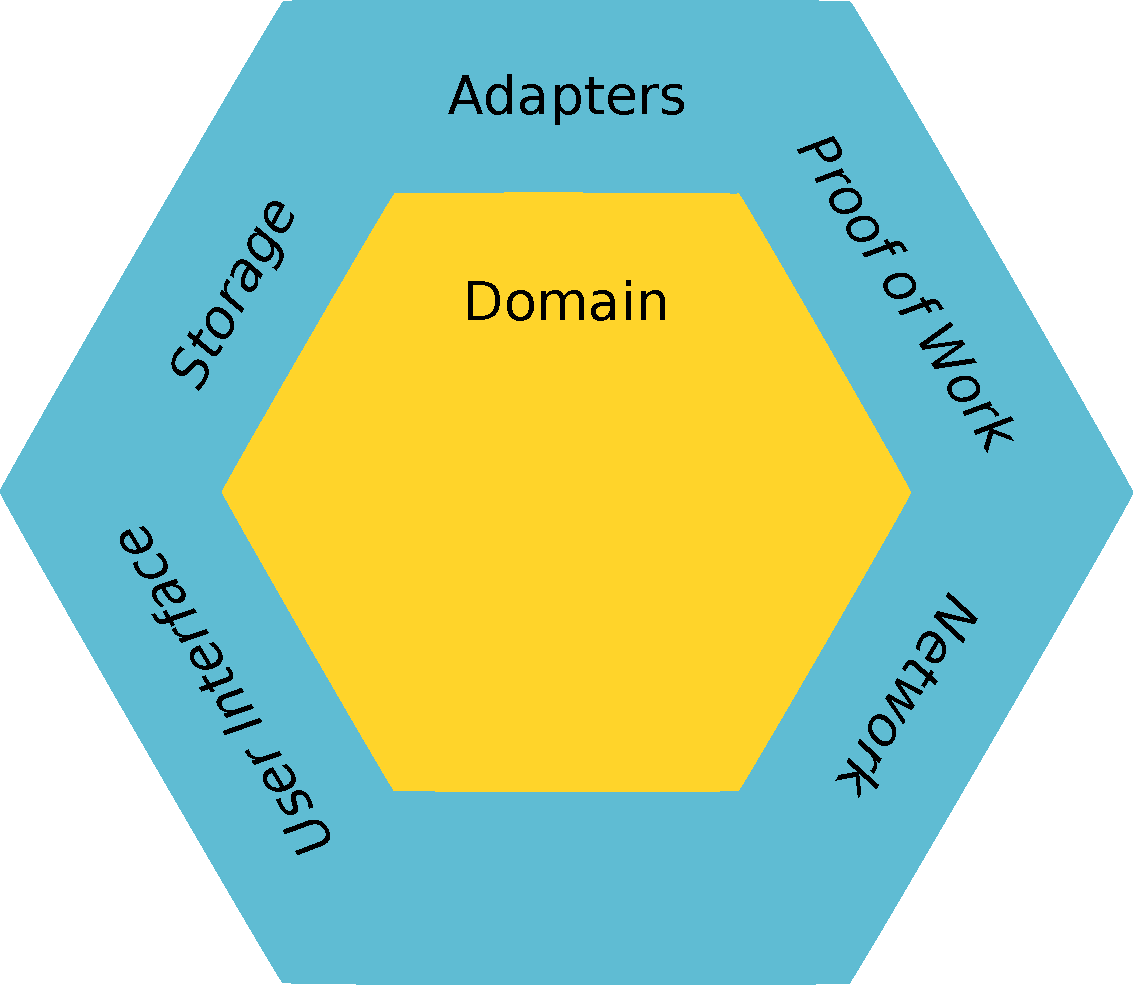
\includegraphics[width=\textwidth]{images/ports_and_adapters.pdf}

  The big advantage of this approach is that it's easy to test the core as well as each adapter by itself.


  \subsection{Network Management}


  \section{Usage}

  TODO


  \section{Discussion}


  \appendix
  \addcontentsline{toc}{section}{Appendix}
  \section*{Appendix}
  \renewcommand{\thesubsection}{\Alph{subsection}}


  \subsection{JavaDoc Documentation}


  \subsection{Literature}


\end{document}